% Options for packages loaded elsewhere
\PassOptionsToPackage{unicode,}{hyperref}
\PassOptionsToPackage{hyphens}{url}
%
\documentclass[
  ]{scrartcl}
\usepackage{amsmath,amssymb}
\usepackage{iftex}
\ifPDFTeX
  \usepackage[T1]{fontenc}
  \usepackage[utf8]{inputenc}
  \usepackage{textcomp} % provide euro and other symbols
\else % if luatex or xetex
  \usepackage{unicode-math} % this also loads fontspec
  \defaultfontfeatures{Scale=MatchLowercase}
  \defaultfontfeatures[\rmfamily]{Ligatures=TeX,Scale=1}
\fi
\usepackage{lmodern}
\ifPDFTeX\else
  % xetex/luatex font selection
\fi
% Use upquote if available, for straight quotes in verbatim environments
\IfFileExists{upquote.sty}{\usepackage{upquote}}{}
\IfFileExists{microtype.sty}{% use microtype if available
  \usepackage[]{microtype}
  \UseMicrotypeSet[protrusion]{basicmath} % disable protrusion for tt fonts
}{}
\makeatletter
\@ifundefined{KOMAClassName}{% if non-KOMA class
  \IfFileExists{parskip.sty}{%
    \usepackage{parskip}
  }{% else
    \setlength{\parindent}{0pt}
    \setlength{\parskip}{6pt plus 2pt minus 1pt}}
}{% if KOMA class
  \KOMAoptions{parskip=half}}
\makeatother
\usepackage{xcolor}
\usepackage{longtable,booktabs,array}
\usepackage{calc} % for calculating minipage widths
% Correct order of tables after \paragraph or \subparagraph
\usepackage{etoolbox}
\makeatletter
\patchcmd\longtable{\par}{\if@noskipsec\mbox{}\fi\par}{}{}
\makeatother
% Allow footnotes in longtable head/foot
\IfFileExists{footnotehyper.sty}{\usepackage{footnotehyper}}{\usepackage{footnote}}
\makesavenoteenv{longtable}
\usepackage{graphicx}
\makeatletter
\def\maxwidth{\ifdim\Gin@nat@width>\linewidth\linewidth\else\Gin@nat@width\fi}
\def\maxheight{\ifdim\Gin@nat@height>\textheight\textheight\else\Gin@nat@height\fi}
\makeatother
% Scale images if necessary, so that they will not overflow the page
% margins by default, and it is still possible to overwrite the defaults
% using explicit options in \includegraphics[width, height, ...]{}
\setkeys{Gin}{width=\maxwidth,height=\maxheight,keepaspectratio}
% Set default figure placement to htbp
\makeatletter
\def\fps@figure{htbp}
\makeatother
\setlength{\emergencystretch}{3em} % prevent overfull lines
\providecommand{\tightlist}{%
  \setlength{\itemsep}{0pt}\setlength{\parskip}{0pt}}
\setcounter{secnumdepth}{-\maxdimen} % remove section numbering
% definitions for citeproc citations
\NewDocumentCommand\citeproctext{}{}
\NewDocumentCommand\citeproc{mm}{%
  \begingroup\def\citeproctext{#2}\cite{#1}\endgroup}
\makeatletter
 % allow citations to break across lines
 \let\@cite@ofmt\@firstofone
 % avoid brackets around text for \cite:
 \def\@biblabel#1{}
 \def\@cite#1#2{{#1\if@tempswa , #2\fi}}
\makeatother
\newlength{\cslhangindent}
\setlength{\cslhangindent}{1.5em}
\newlength{\csllabelwidth}
\setlength{\csllabelwidth}{3em}
\newenvironment{CSLReferences}[2] % #1 hanging-indent, #2 entry-spacing
 {\begin{list}{}{%
  \setlength{\itemindent}{0pt}
  \setlength{\leftmargin}{0pt}
  \setlength{\parsep}{0pt}
  % turn on hanging indent if param 1 is 1
  \ifodd #1
   \setlength{\leftmargin}{\cslhangindent}
   \setlength{\itemindent}{-1\cslhangindent}
  \fi
  % set entry spacing
  \setlength{\itemsep}{#2\baselineskip}}}
 {\end{list}}
\usepackage{calc}
\newcommand{\CSLBlock}[1]{\hfill\break\parbox[t]{\linewidth}{\strut\ignorespaces#1\strut}}
\newcommand{\CSLLeftMargin}[1]{\parbox[t]{\csllabelwidth}{\strut#1\strut}}
\newcommand{\CSLRightInline}[1]{\parbox[t]{\linewidth - \csllabelwidth}{\strut#1\strut}}
\newcommand{\CSLIndent}[1]{\hspace{\cslhangindent}#1}
\ifLuaTeX
\usepackage[bidi=basic]{babel}
\else
\usepackage[bidi=default]{babel}
\fi
\babelprovide[main,import]{american}
% get rid of language-specific shorthands (see #6817):
\let\LanguageShortHands\languageshorthands
\def\languageshorthands#1{}
\raggedbottom % or \flushbottom
% keep figures where there are in the text
\usepackage{float} 
\floatplacement{figure}{H}
% add custom hyphentation rules
\hyphenation
{%
  Hyphenate-me-like-this
  Dontyoueverhyphenateme
}%
\ifLuaTeX
  \usepackage{selnolig}  % disable illegal ligatures
\fi
\usepackage{bookmark}
\IfFileExists{xurl.sty}{\usepackage{xurl}}{} % add URL line breaks if available
\urlstyle{same}
\hypersetup{
  pdftitle={MedMamba: Toward Efficient and Accurate Medical Image Classification},
  pdfauthor={Shany Herskovits; Ofir Nahshon; Michael Berger},
  pdflang={en-US},
  hidelinks,
  pdfcreator={LaTeX via pandoc}}

\title{MedMamba: Toward Efficient and Accurate Medical Image
Classification}
\usepackage{etoolbox}
\makeatletter
\providecommand{\subtitle}[1]{% add subtitle to \maketitle
  \apptocmd{\@title}{\par {\large #1 \par}}{}{}
}
\makeatother
\subtitle{With Rejection}
\author{\href{mailto:shanyh@gmail.com}{Shany
Herskovits} \and \href{mailto:ofiranava@gmail.com}{Ofir
Nahshon} \and \href{mailto:michael.berger.e@gmail.com}{Michael Berger}}
\date{18 March 2025}

\begin{document}
\maketitle
\begin{abstract}
In this project, we bla bla bla Our demo is avaliable on Github on this
link: \url{https://github.com/vodkolav/MedMamba}
\end{abstract}



\renewcommand*\contentsname{Contents}
{
\setcounter{tocdepth}{1}
\tableofcontents
}
\section{Introduction}\label{introduction}

Content\\
this is how you make citations: MedMamba{[}yue2024medmamba{]} the
yue2024medmamba part must be an id in references in frontmatter block
above

\section{Problem description}\label{problem-description}

Content

\section{Data Description}\label{data-description}

Content

\section{Preprocessing}\label{preprocessing}

Content

\section{Base model description}\label{base-model-description}

Content\\
then inline formula: \(l/2 Hz\)

Embedding images:\\
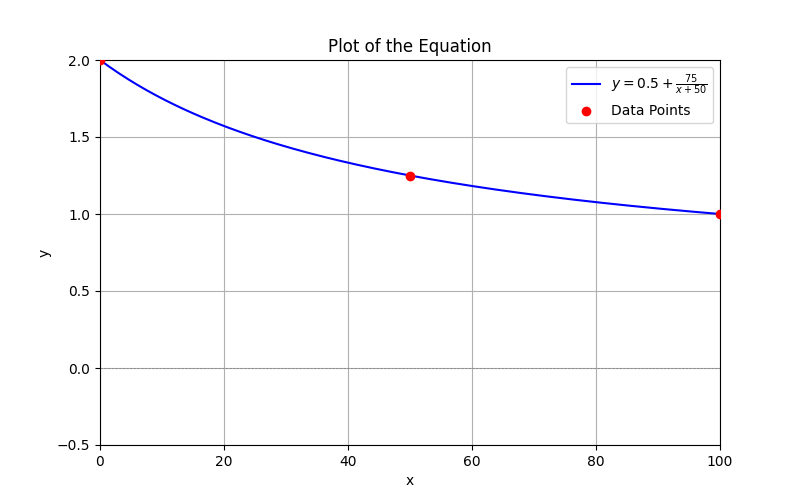
\includegraphics{../Equation_plot3.png}

big formula, will be centered on page:

\[\arg\min_{G_\theta} \|v_k - G(z_k, k, \mathcal{F}_{\text{enc}}(X_l); \theta)\|_2^2\]

another formula example:

\[v_t = \sqrt{\bar{\alpha}_t} \epsilon - \sqrt{1 - \bar{\alpha}_t} x_0\]

To put greek letters in text, just use inline formula : \(\epsilon\) and
\(x_0\).

\section{Rejection model description}\label{rejection-model-description}

Content

\section{Model parameters and how it's
trained}\label{model-parameters-and-how-its-trained}

Content

\section{Experiments}\label{experiments}

Content

\section{Results}\label{results}

Content\\
a markdown table:

\begin{longtable}[]{@{}ll@{}}
\toprule\noalign{}
Model & LSD \\
\midrule\noalign{}
\endhead
\bottomrule\noalign{}
\endlastfoot
GT-Mel & 0.61 \\
Unprocessed & 1.99-4.25 \\
NVSR-DNN & 1.13- 1.67 \\
NVSR-ResUNet & 1.7- 0.95 \\
AUDIOSR & 0.99- 0.73 \\
AUDIOSR + Noise (our model) & 2 - 1.2 \\
\end{longtable}

\section{Conclusion}\label{conclusion}

Content

\section{References}\label{references}

\phantomsection\label{refs}
\begin{CSLReferences}{0}{1}
\end{CSLReferences}



\end{document}
